

\tikzset{every picture/.style={line width=0.75pt}} %set default line width to 0.75pt

\begin{tikzpicture}[x=0.75pt,y=0.75pt,yscale=-1,xscale=1]
%uncomment if require: \path (0,239.75); %set diagram left start at 0, and has height of 239.75

%Straight Lines [id:da9129665010836374]
\draw (180,190) -- (480,190) (280,186) -- (280,194)(380,186) -- (380,194) ;


%Straight Lines [id:da2940576875009948]
\draw (180,120) -- (480,120) (280,116) -- (280,124)(380,116) -- (380,124) ;


%Straight Lines [id:da33097894050012455]
\draw (180,80) -- (480,80) (280,76) -- (280,84)(380,76) -- (380,84) ;


%Straight Lines [id:da12784184495069784]
\draw (180,40) -- (480,40) (280,36) -- (280,44)(380,36) -- (380,44) ;


%Straight Lines [id:da17947621369901245]
\draw [dashed] (280,40) -- (280,190) ;


%Straight Lines [id:da7306352886260447]
\draw [dashed] (380,40) -- (380,190) ;



% Text Node
\draw (505,39.5) node {$x-1$};
% Text Node
\draw (505,79.5) node {$x-1$};
% Text Node
\draw (492,119.5) node {$x$};
% Text Node
\draw (427.5,29.5) node {$+$};
% Text Node
\draw (227.5,30.5) node {$-$};
% Text Node
\draw (380,28.5) node {$1$};
% Text Node
\draw (280,28.5) node {$0$};
% Text Node
\draw (427.5,69.5) node {$+$};
% Text Node
\draw (427.5,109.5) node {$+$};
% Text Node
\draw (427.5,179.5) node {$+$};
% Text Node
\draw (332.5,109.5) node {$+$};
% Text Node
\draw (332.5,179.5) node {$+$};
% Text Node
\draw (227.5,69.5) node {$-$};
% Text Node
\draw (227.5,109.5) node {$-$};
% Text Node
\draw (227.5,179.5) node {$-$};
% Text Node
\draw (332.5,29.5) node {$-$};
% Text Node
\draw (332.5,69.5) node {$-$};
% Text Node
\draw (513.5,187.5) node {$\dfrac{( x-1)^{2}}{x}$};
% Text Node
\draw (280,201.5) node {$0$};
% Text Node
\draw (380,202.5) node {$1$};

% Intervalo aberto
\draw[fill=white] (280,40) circle (3.25);
% Intervalo aberto
\draw[fill=white] (280,80) circle (3.25);
% Intervalo aberto
\draw[fill=white] (280,120) circle (3.25);
% Intervalo aberto
\draw[fill=white] (280,190) circle (3.25);


\end{tikzpicture}
